\documentclass{standalone}
\usepackage{tikz}
\usetikzlibrary{calc}
\usetikzlibrary{shapes,arrows,positioning,decorations.pathreplacing}
\usepackage{amsmath}


\tikzstyle{startstop} = [rectangle, rounded corners, text width=2cm,text centered, minimum height=1cm, draw=black]
\tikzstyle{io} = [trapezium, trapezium left angle=70,trapezium right angle=110, text width=3.3cm, minimum height=1cm, text centered, draw=black, trapezium stretches=true]
\tikzstyle{process} = [rectangle, text width=3.3cm, minimum height=1cm, text centered, draw=black]
\tikzstyle{decision} = [diamond, text width=3.3cm, minimum height=1cm, text centered, draw=black]

\begin{document}
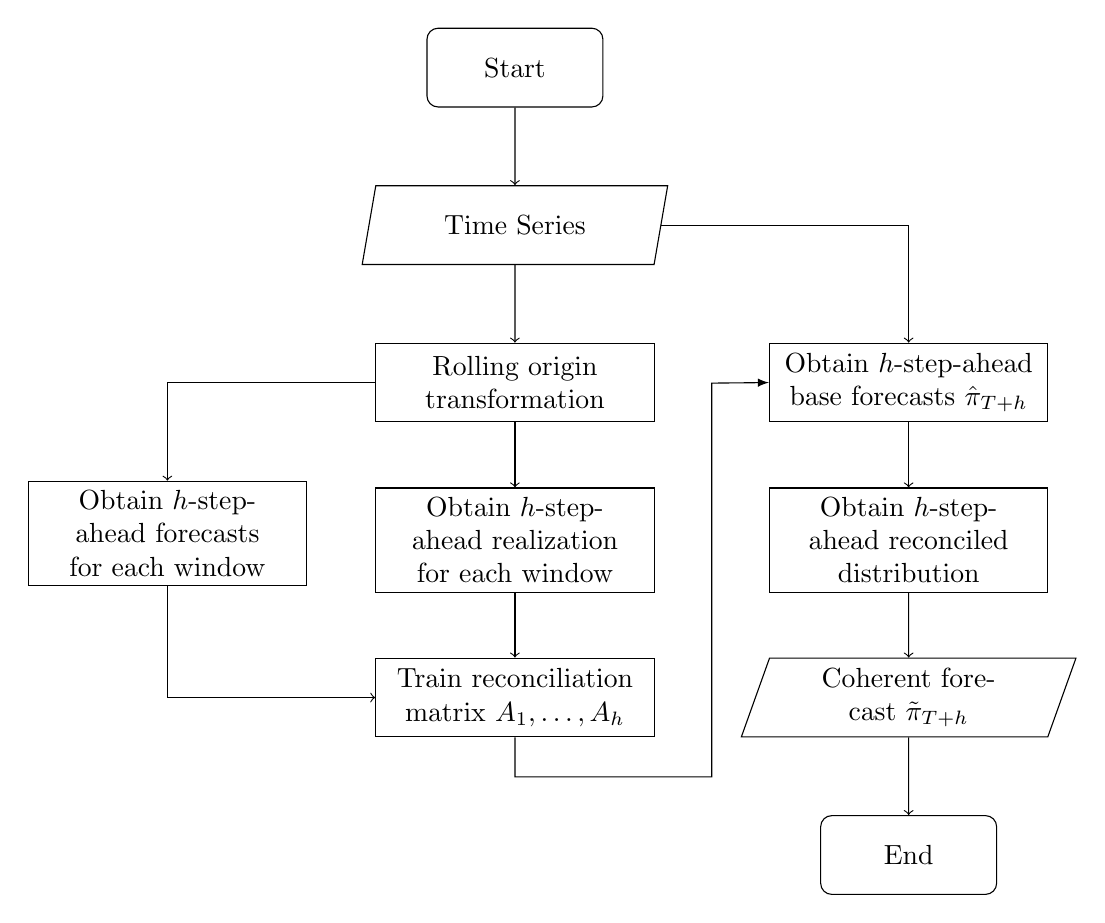
\begin{tikzpicture}[node distance=2cm]
    
    \node(start)[startstop]{Start};
    \node(in)[io, below of=start]{Time Series};

    \node(rollingorigin)[process, below of=in]{Rolling origin transformation};

    \node(train1)[process, below left of=rollingorigin, xshift=-3cm, yshift=-0.5cm]{Obtain $h$-step-ahead forecasts for each window};
    \node(train2)[process, below of=rollingorigin]{Obtain $h$-step-ahead realization for each window};

    \node(train3)[process, below of=train2]{Train reconciliation matrix $A_1,\dots,A_h$};

    \node(forecast1)[process,right of=rollingorigin, xshift=3cm]{Obtain $h$-step-ahead base forecasts $\hat{\mathbf{\pi}}_{T+h}$};
    \node(forecast2)[process, below of=forecast1]{Obtain $h$-step-ahead reconciled distribution};
    \node(output)[io, below of=forecast2]{Coherent forecast $\tilde{\mathbf{\pi}}_{T+h}$};
    \node(end)[startstop, below of=output]{End};

    \draw[->] (start) edge (in) 
        (in) edge (rollingorigin) ;
    \draw[->] (rollingorigin) -| (train1) ;
    \draw[->] (rollingorigin.south) -| (train2) ;

    \draw[->] (train1) |- (train3);
    \draw[->] (train2.south) -| (train3);
    \draw[->] (in.east) -| (forecast1.north);
    \draw[-latex] (train3.south) |- ++(2.5,-0.5) -- ++(0,5.0) -- (forecast1.west);
    \draw[->] (forecast1) -- (forecast2);


    \draw[->] (forecast2) -- (output);
    \draw[->] (output) -- (end);

    % Stage 1 nodes
    % \node [block] (windowing) {Transform time series into windows using rolling forecast origin strategy};
    % \node [block, below left=1.5cm and 0.5cm of windowing] (base-forecasts) {Generate $h$-step-ahead base forecasts $\hat{\boldsymbol{\pi}}$};
    % \node [block, below right=1.5cm and 0.5cm of windowing] (realization) {Obtain corresponding realization $\mathbf{z}$};
    % \node [block, below=2.5cm of windowing] (optimal-A) {Calculate optimal reconciliation matrix $\mathbf{A}$};
    
    % % Stage 2 nodes
    % \node [block, right=3cm of windowing] (coherent-distribution) {Obtain coherent joint distribution};
    % \node [block, below of=coherent-distribution] (multi-step) {Obtain multi-step ahead forecasts};
    
    % % Stage labels
    % \coordinate[left=0.5cm of windowing.west] (stage1-left);
    % \coordinate[left=0.5cm of optimal-A.west] (stage1-right);
    % \node [align=left, text width=2cm, above=0.25cm of stage1-left] {Training Stage};
    
    % \draw [decorate,decoration={brace,amplitude=10pt,mirror}] (stage1-left) -- (stage1-right) node[midway, xshift=-1.5cm, yshift=0cm] {};
    
    % \coordinate[left=0.5cm of coherent-distribution.west] (stage2-left);
    % \coordinate[left=0.5cm of multi-step.west] (stage2-right);
    % \node [align=left, text width=2cm, above=0.25cm of stage2-left] {Forecasting Stage};
    
    % \draw [decorate,decoration={brace,amplitude=10pt,mirror}] (stage2-left) -- (stage2-right) node[midway, xshift=-1.5cm, yshift=0cm] {};
    
    % % Lines
    % \path [line] (windowing) -- (base-forecasts);
    % \path [line] (windowing) -- (realization);
    % \path [line] (base-forecasts) -- (optimal-A);
    % \path [line] (realization) -- (optimal-A);
    % \path [line] (optimal-A) -- (coherent-distribution);
    % \path [line] (coherent-distribution) -- (multi-step);
    
\end{tikzpicture}
\end{document}
